\cleardoublepage

\section{Projects}

\begin{FlushLeft}
\\[1in]
\subsection{elm-bblsort}
\\[0.1in]
\subsubsection{Assigned Task}
Replicate the implementation of the \href{https://algodynamics.io/bubblesort/machines/bubblesortManual.html}{bubble sort exercise} present in the Algodynamics site.
\\[0.5in]
\subsubsection{Implementation}
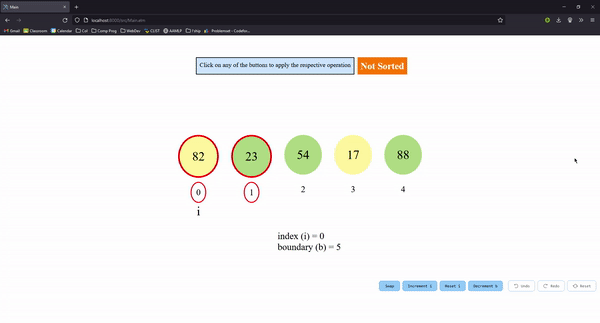
\includegraphics[width=5in]{imgs/bbl-sort.png}

\begin{itemize}
    \item Unique messages are displayed depending on the users chosen operation. For example, if the user is deviating from the bubble sort algorithm, a message is displayed to warn the user. 
    \item Elements in the correct position are highlighted in green, giving a clear indication on which elements are correctly placed. 
    \item Transitions were added too, to make it more visually appealing. 
    \item Utilized \href{https://package.elm-lang.org/packages/algodynamics-iiith/core/latest/}{Core Package} to include the Undo, Redo and Reset features. 
\end{itemize}

\cleardoublepage

\subsubsection{Learning Outcomes}
\begin{itemize}
    \item Got a good understanding of how elm code should be structured.
    \item Learnt to utilize other packages in the project, obtained from \href{https://package.elm-lang.org/}{elm packages} site.
    \item Familiarized myself with the significance of model-view-update architecture in Elm. 
\end{itemize}

\\[1in]
\subsection{elm-calci}
\\[0.1in]
\subsubsection{Assigned Task}
Implement a simple calculator using Elm. 
\\[0.5in]
\subsubsection{Implementation}

\begin{figure}[h]
    \centering
    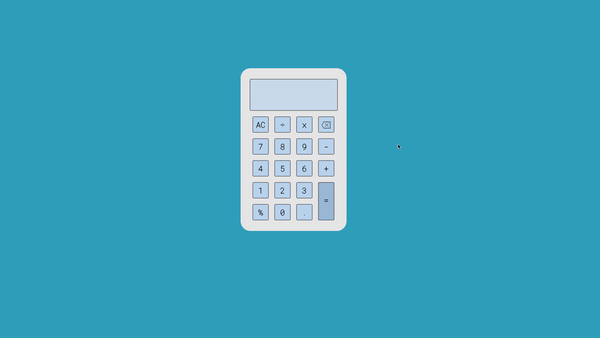
\includegraphics[width=5in]{imgs/elm-calci-1.png}
    \caption{Implementation without template code}
\end{figure}

\begin{figure}[h]
    \centering
    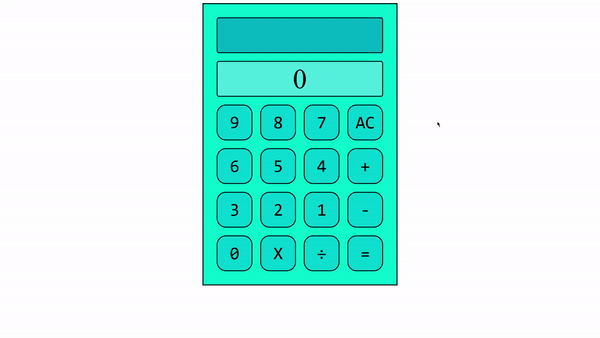
\includegraphics[width=5in]{imgs/elm-calci-2.png}
    \caption{Implementation with template code}
\end{figure}


\begin{itemize}
    \item In the implementation without the template code, the display shows two values - one of which shows the input entered by the user, and the other shows the history of calculations carried out. 
    \item But it had a drawback - the operations carried out by the user was not in accordance with BODMAS rule. So there was a scope of inaccuracy. 
    \item This drawback was rectified with the help of the second implementation. 
    \item It was also ensured that the button SVG's are generated in a single SVG canvas through the aid of a recursive function, which will come in handy in the next project.
    \item Attributes to modify the button styling, dimensions and arrangement have also been added. 
\end{itemize}

\\[0.5in]

\subsubsection{Learning Outcomes}
\begin{itemize}
    \item Grasped a good understanding of utilizing SVG with Elm, to elements with user-desired configuration. \item Learnt how to make custom attributes, which can be assigned a default value if the user chooses not to enter their own value for the same.  
\end{itemize}
\\[0.5in]

\subsection{elm-dagre}
\\[0.1in]
\subsubsection{Assigned Task}
Document the working of \href{https://package.elm-lang.org/packages/goyalarchit/elm-dagre/}{elm-dagre} package and showcasing the significance of some of the modules present in the package. 
\\[0.5in]
\subsubsection{Implementation}
Descriptions of the attributes and modules can be found in \href{https://github.com/kmvolv/elm-dagre-task/blob/main/task.md}{this} markdown file. 
\\[0.5in]
\subsubsection{Learning Outcomes}
\begin{itemize}
    \item Was able to get an idea about the various attributes and drawers used to generate the visualization for the user specified graph.
    \item Got an understanding on how an elm package is made, which is what is to be done in the next task. 
\end{itemize}
\\[1in]
\subsection{elm-array-view}
\\[0.1in]
\subsubsection{Assigned Task}
Create code which generates the visualization for a user-specified array and publish a package on the same. 
\cleardoublepage
\subsubsection{Implementation}
\begin{figure}[h]
    \centering
    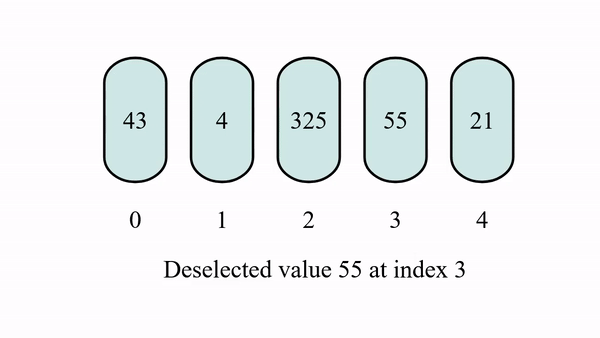
\includegraphics[width=5in]{imgs/elm-arr-1.png}
    \caption{Implementation without elm-dagre}
\end{figure}

\begin{figure}[h]
    \centering
    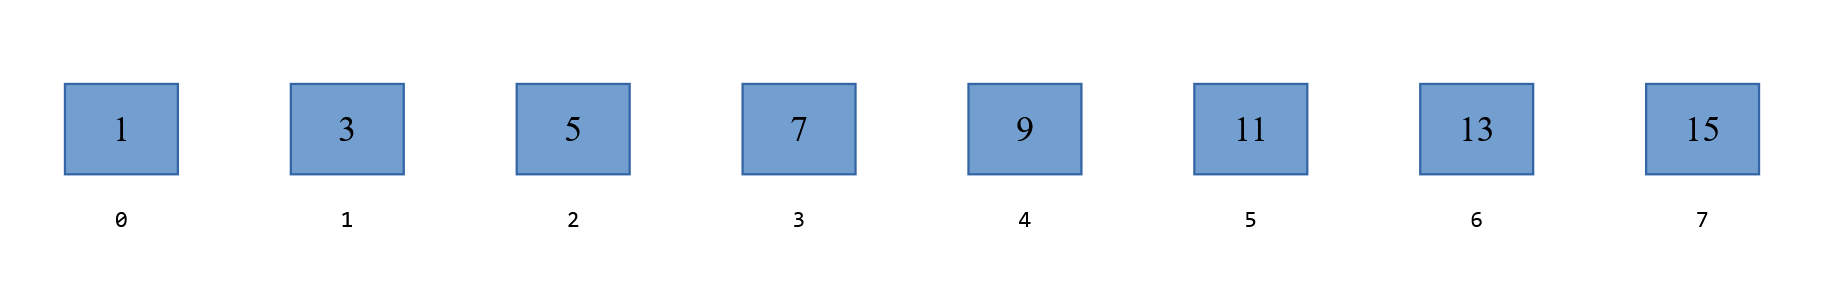
\includegraphics[width=5in]{imgs/elm-arr-2.png}
    \caption{Implementation with elm-dagre}
\end{figure}

\begin{itemize}
    \item A user specified array is visualized with the help of this module. 
    \item Through added user attributes, the dimensions, shape and positioning of index labels can be modified. 
    \item The first implementation has a drawback of not having a wrap feature and having static index label positions. Also, the array containers are not individually configurable. 
    \item These drawbacks were taken care of in the second implementation, in which the elm-dagre package is utilized. 
    \item A custom drawer is created in order to avoid any confusion with the graph attributes.
    \item Positioning of index labels can be set at any position by specifying the desired X and Y co-ordinates. 
    \item Additional features such as setting a limit of the number of elements that can be present in a single row can also be added by the user by making minor tweaks to the drawer function. 
\end{itemize}

\subsubsection{Learning Outcomes}
\begin{itemize}
    \item With the help of what we've learnt from the previous projects, we were able to implement this array visualization function. 
    \item Learnt about the process involved in deploying an elm package and how one can properly document it. \item Grasped valuable insight on making simple and well structured code so that one can easily make tweaks to it if they need to. 
\end{itemize}

\end{FlushLeft}